\chapter{Introduction to Turbulent Combustion} % (fold)
\label{cha:turbulent_combustion}
%
\lettrine[lines=3, lhang=0.05]{C}{ombustion} is one of the cornerstones of our
civilization.
%
It provides light in a candle or carries objects into space in a rocket engine.
%
The majority of high-tech combustion processes occur under turbulent conditions.
%
The nature of turbulent flow, and therefore also turbulent combustion, is still
being actively studied by the scientific community.
%
Reducing the pollutant emissions and increasing the efficiency of combustion
processes is essential in todays world where we are confronted more and more
often with the realization that our resources are finite and the damage we do to
our environment can not easily be undone.
%

%
Simulations are an invaluable tool in the design of improved combustion
processes.
%
They allow to test different setups quickly and for a relatively low cost.
%
Efficient simulations need models of the relevant physical and chemical
processes.
%
As the demands on the accuracy of such models rises, more detailed insight into
the low-level phenomena of turbulent combustion is needed.
%
Obtaining this insight via experiments is challenging.
%
Often only a small number of variables can be observed at the same time and
observations are frequently limited to a \ac{2D} slice.
%

%
Another approach is \acf{DNS}, which is sometimes referred to as a ``numerical
experiment''.
%
In \ac{DNS}, the Navier-Stokes equation is directly solved on a very fine grid,
without using any higher-level modeling assumptions.
%
This is computationally very expensive, which is why \ac{DNS} is typically
performed on supercomputers using hundreds or thousands of cores.
%
In the simulation, all variables are available in full spatial and temporal
resolution.
%

%
Analyzing the data from such simulations poses a different challenge.
%
Due to the high spatial and temporal resolution, the raw data produced by a
single \ac{DNS} run can range from Terabytes to Petabytes.
%
Data of this size can not be written to disk or transferred over a network in a
reasonable amount of time, even if the enormous storage space that is required
was available.
%
This limits the post-analysis of the data to spatially or temporally downsampled
versions which lose a lot of important information.
%
In recent years, the subject of \emph{in-situ} analysis and visualization has
therefore gained popularity.
%
The idea is to process the data while it is still in memory during the
simulation.
%
The raw data is then discarded and only the results, which are typically much
smaller in size, are stored on disk.
%

%
This thesis contains two new in-situ focused approaches for analysis and
visualization of turbulent combustion \ac{DNS}.
%
To provide some important context, this chapter provides a short introduction
into the field of turbulent combustion research, the basics of turbulent
combustion modeling and simulation, and an overview of relevant research
concerning in-situ and post-processing of turbulent combustion data in
particular and large-scale simulations in general.
%

\section{Combustion} % (fold)
\label{sec:combustion}
%
Combustion is the exothermic chemical reaction of a fuel and an oxidizer into
oxidized products and heat.
%
We will only concern ourselves with the combustion of gases, which is the
most common case used in industrial applications.
%
The oxidizer is usually oxygen, while fuels can range from simple ones such as
hydrogen or methane to complex organic fuels.
%

%
A combustion process is a complex system of elementary chemical reactions
transforming various chemical species into each other while absorbing or
releasing heat.
%
It involves reactants and products but also various intermediate species.
%
These intermediates can be more or less stable and are often radicals with
unpaired electrons.
%
The reaction rate of each elementary reaction in an infinitesimal volume is
dependent on the amounts (\ie, mass) of the different chemical species as well
as the current temperature.
\Todo{define mass fractions and density}
%
The process can additionally be influenced by the diluting presence of inert
gases that do not participate in the reaction.
%

%
The chemical reactions in a flame are intrinsically linked to the fluid motion
of the gas.
%
As the gas is deformed and transported by the flow, the local concentration and
temperature gradients change, which in turn control the diffusion of chemical
species and heat.
%
Through diffusion, the local mixture and temperature changes, which in turn
influences the reaction rates.
%
As the chemical reactions produce or consume heat, the gas expands or contracts,
which in turn influences the fluid's velocity (the expanded gas has to go
somewhere) and viscosity (molecules that are farther away from each other
interact less).
%
This again influences the mixing and transport of the gas, and so the cycle goes
on.
%

%
Gaseous combustion can be classified by the type of flow and the mixing of
reactants.
%
Is the flow laminar or turbulent, and are fuel and oxidizer premixed or
non-premixed?
%
We will discuss the characteristics of flames in each of these regimes in the
following sections.
%
This discussion is largely based on the book ``Theoretical and Numerical
Combustion'' by Poinsot and Veynante~\cite{Poinsot2012}.
%
\subsection{Laminar Flames} % (fold)
\label{sub:laminar_flames}
%
If the reacting gases in a flame move at low velocities, the flow is often
laminar.
%
Laminar flow is characterized by the absence of eddies or vortices.
%
Layers of the fluid slide past each other without significant mixing.
%
In many cases, the flow is steady in this regime.
%

%
Even though laminar flames are the exception in industrial applications, their
simplicity and deterministic behavior makes them an ideal basis for the
theoretical study of combustion processes.
%
They are the reference case that turbulent combustion is compared against and
that turbulent combustion models are derived from.
%
\subsubsection{Laminar Premixed Flames} % (fold)
\label{ssub:laminar_premixed_flames}
%
In a premixed flame, fuel and oxidizer are brought into a uniform mixture before
ignition.
%
The defining feature of premixed combustion is the flame front that propagates
into the fresh gases and leaves behind hot combustion products.
%
In the simplest case, the flame front is planar and travels along its normal
direction.
%
In this case, the phenomenon is essentially one-dimensional (see
\cref{fig:premixed_profiles}).
%
\begin{figure}[t]
    \centering
    % \MissingFigure{\ac{1D} profiles of an ideal premixed flame}
    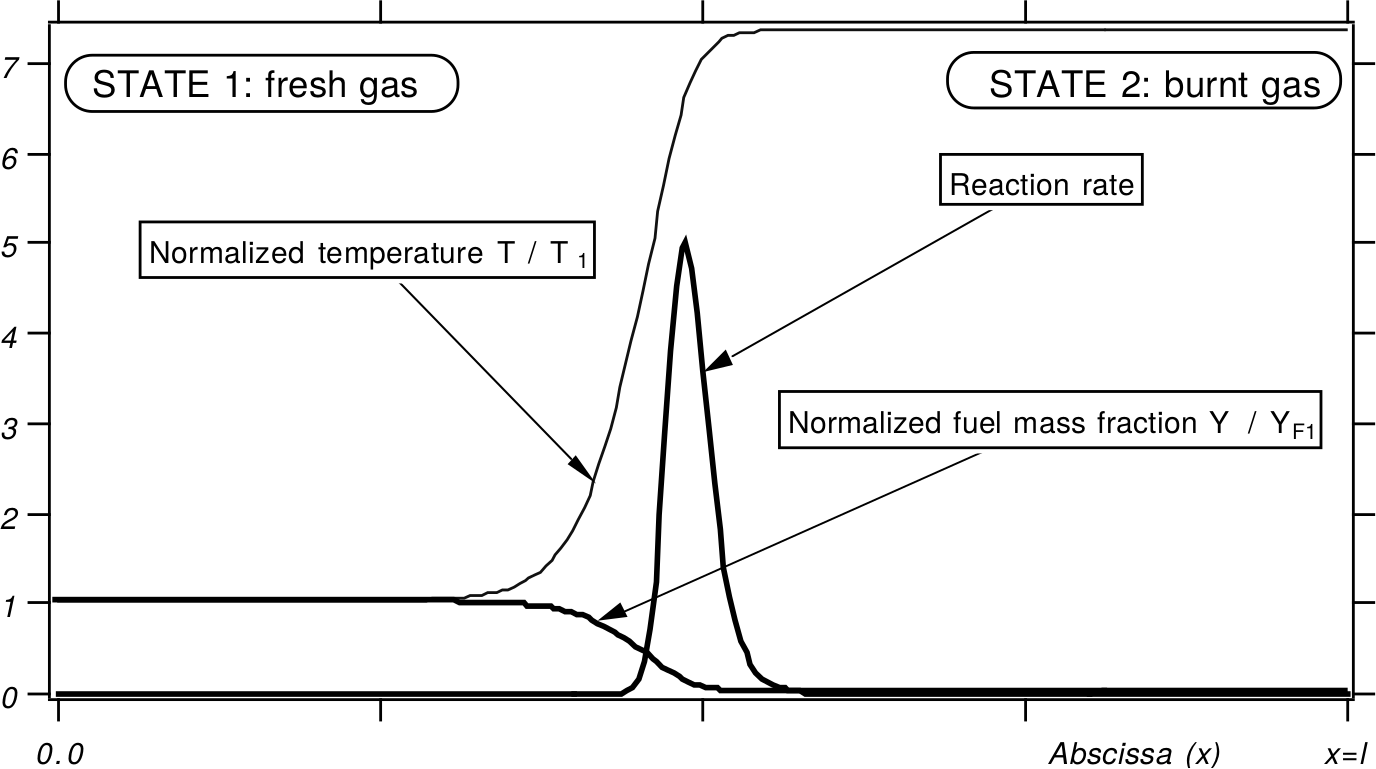
\includegraphics[width=\textwidth]{figures/1D_premixed_flame.png}
    \caption{Basic configuration of a one-dimensional laminar premixed flame.
    Image source: Poinsot and Veynante~\cite{Poinsot2012}}
    \label{fig:premixed_profiles}
    \Suggestion[inline]{Recreate in tikz?}
\end{figure}
%
The profiles of the combustion variables along the normal direction show high
concentrations of fuel and oxidizer on the fresh gas side and high combustion
product concentrations and temperature on the burnt gas side.
%
In between the two extrema is the flame front that shows the gradual transition
between fresh and burnt gases.
%
The concentration of intermediate species is highest in the flame front.
%
Intermediates generally do not occur in the fresh gases, but some radicals may
exist on the burnt gas side due to dissociation of combustion products at high
temperatures.
%
\begin{figure}[t]
    \centering
    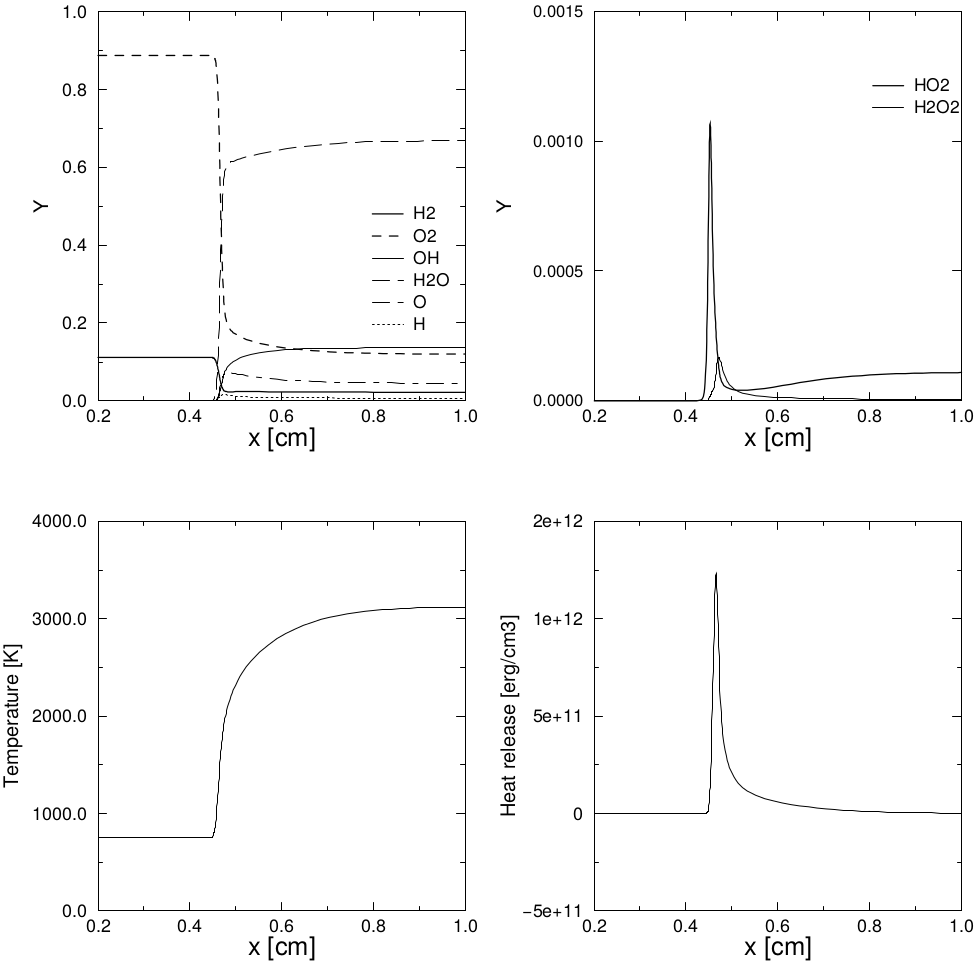
\includegraphics[width=\textwidth]{figures/laminar_flame.png}
    \caption{Profiles of species (Y), temperature and heat release of a
    laminar premixed \ce{H2}-\ce{O2} flame. Image source: Poinsot and
    Veynante~\cite{Poinsot2012}}
    \label{fig:laminar_premixed_profiles}
\end{figure}

%
The characteristic properties of a premixed flame front are \emph{flame speed},
\emph{flame stretch}, and \emph{flame thickness}.
%
These three quantities depend on each other and the underlying flow field.
%

%
The flame speed is the speed at which the flame front travels.
%
It can be expressed relative to a laboratory frame of reference, or relative to
the flow. \Todo{mention in surface tracking chapter which definition is used}
%
Sometimes, it is also expressed as the speed at which fresh gases are turned
into combustion products.
%
The flame speed can vary considerably along the surface of a flame, and
depending on conditions, the flame front can travel against the flow at
considerable speeds.
%

%
The flame thickness describes the width of the reaction zone normal to the flame
front.
%
Depending on the application, it is determined in different ways.
%
One common definition uses the slope at the point of highest temperature
gradient.
%
Another one is based on the distance between the isosurfaces of minimum and
maximum temperature.
%
Different alternative definitions exist as well, some of them based on radical
species.
%
The flame thickness is inversely proportional to the flame speed.
%
A thinner flame travels more quickly and slow-moving flames tend to be thicker.
%
Flame thickness is an essential measurement for combustion simulations, as it
determines the grid resolution necessary to resolve the flame front.
%

%
Both flame speed and flame thickness are dependent on the chemical reaction
taking place and the stretch of the flame front.
%
Flame stretch is the change in surface area an infinitesimal element of the
(idealized) flame surface experiences over an infinitesimal time interval.
%
It can be induced by a non-uniform flow, but also by the expansion or
contraction a curved flame front experiences due to its propagation in normal
direction.
%
\Cref{fig:stretched_premixed_flames} shows some examples of stretched laminar
premixed flames.
%
If the flame experiences positive stretch, it is tangentially expanded and
compressed in normal direction.
%
This decreases the flame thickness and feeds new fresh gases to the reaction,
which increases the flame speed.
%
However, it also increases heat dissipation.
%
If the flame is stretched too quickly, this can lead to quenching.
%
Negative stretch (compression) leads to less fresh gas being transported near
the reaction zone, which increases the flame thickness and reduces flame speed.
%
\begin{figure}[tp]
    \centering
    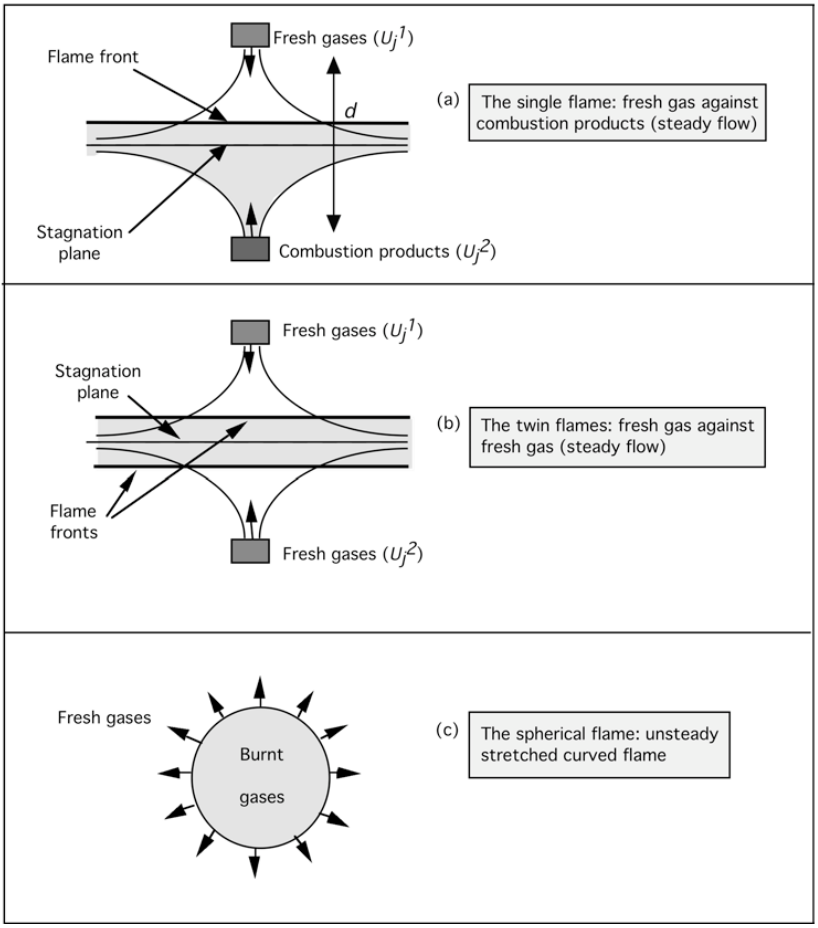
\includegraphics[width=\textwidth]{figures/stretched_premixed_flames.png}
    \caption{Examples of stretched laminar premixed flames. Image source:
    Poinsot and Veynante~\cite{Poinsot2012}}
    \label{fig:stretched_premixed_flames}
\end{figure}

%
Due to their defining characteristic for the behavior of the flame, flame speed,
thickness and stretch are the basis for a lot of combustion models, and a focus
of study in many combustion experiments and -simulations.
%
% subsubsection laminar_premixed_flames (end)
%
\subsubsection{Laminar Non-Premixed (Diffusion) Flames} % (fold)
\label{ssub:laminar_diffusion_flames}
%
In non-premixed combustion, fuel and oxidizer are supplied separately.
%
Combustion can only occur where both mix in a sufficient ratio via diffusion.
%
This is why non-premixed flames are also called diffusion flames.
%
\Cref{fig:laminar_diffusion_profiles} shows a \ac{1D} cross-section of a
typical laminar diffusion flame.
%
\begin{figure}[t]
    \centering
    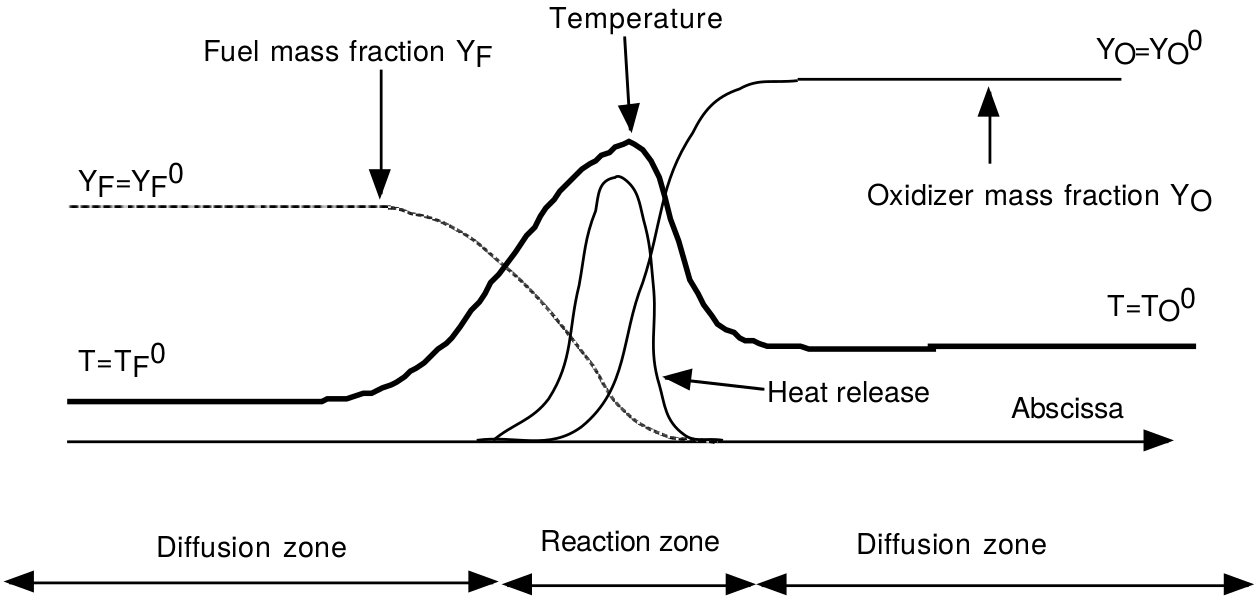
\includegraphics[width=\textwidth]{figures/laminar_diffusion_flame.png}
    \caption{Basic configuration of a one-dimensional laminar diffusion flame.
    Image source: Poinsot and Veynante~\cite{Poinsot2012}}
    \label{fig:laminar_diffusion_profiles}
\end{figure}
%

%
The prototypical example of a diffusion flame is a jet flame where fuel gas is
injected into ambient air and ignited.
%
An example of this type we are all familiar with is the flame of a candle.
%
Wax is evaporated from the wick via the heat of the flame.
%
This fuel gas burns as it comes into contact with ambient air and creates a
laminar diffusion flame.
%
The heat generated from the flame is sufficient to ignite the fresh fuel being
supplied from the wick and sustain the reaction.
%
\Cref{fig:laminar_diffusion_jet} shows a simplified example of such a flame.
%
\begin{figure}[t]
    \centering
    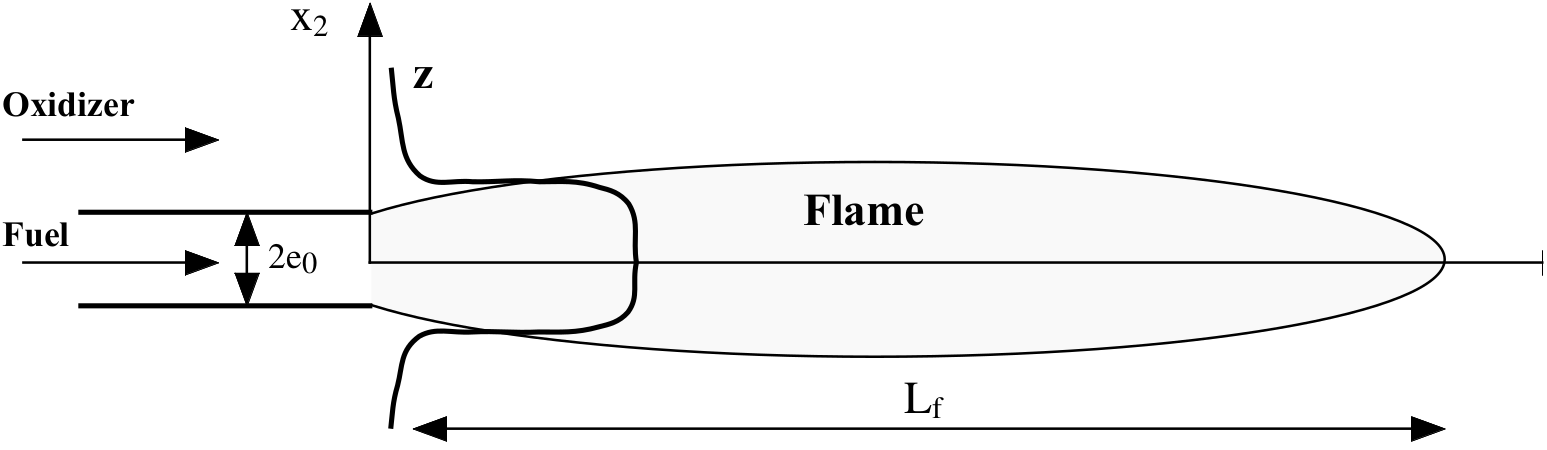
\includegraphics[width=0.8\textwidth]{figures/laminar_diffusion_jet.png}
    \caption{Simple \ac{2D} laminar diffusion jet flame. Image source: Poinsot
    and Veynante~\cite{Poinsot2012}}
    \label{fig:laminar_diffusion_jet}
\end{figure}
%

%
Diffusion flames are easier to set up than premixed flames from a practical
perspective, as no perfect mixing of fuel and oxidizer is required beforehand.
%
They are also safer because they prevent flashbacks into the gas supply.
%
However, it is harder to ensure a clean and complete consumption of fuel in
non-premixed combustion.
%
This is why diffusion flames are generally less efficient and produce more
soot and pollutants that result from suboptimal burning conditions.
%

%
As the conditions for combustion are not satisfied initially, transport and
mixing become the main issues in a non-premixed flame.
%
Fuel and oxidizer need to mix sufficiently to create a combustible mixture.
%
Temperature produced by nearby combustion needs to be high enough to ignite
the mixture.
%
Combustion products need to be transported away from the combustion zone fast
enough to prevent the flame from suffocating, but not too fast to dissipate the
heat required for continued combustion.
%

%
Diffusion flames do not propagate like premixed flames.
%
Their position is fixed at the interface between fuel and oxidizer.
%
For this reason, the speed of the flame is not a relevant quantity in for
analyzing the behavior of diffusion flames.
%
Instead, the defining variable is the mixture fraction between fuel and
oxidizer.
%
The flame is generally strongest where the mixture fraction is near
stoichiometry, \ie, where fuel and oxidizer are mixed in such a ratio that
both are consumed completely by the reaction.
%
Mixture fraction and temperature are the dominating variables controlling a
diffusion flame, which is why simple combustion models are based on these two
quantities.
%

%
Unlike for premixed flames, where it mainly influences the speed of the reaction
and can only quench the flame in extreme cases, diffusion flames are very
sensitive to flame stretch.
%
A certain stretch is necessary to supply fresh gases to the reaction zone and
transport away combustion products that would otherwise suffocate the flame.
%
However, for high flame stretch heat might be dissipated too quickly to sustain
the reaction, leading to extinction.
%

%
Because diffusion flames are much more sensitive to the flow conditions, and
combustion occurs over a wider range of fuel/oxidizer mixture fractions,
modeling and simulating diffusion flames is more challenging than premixed
flames.
%
% subsubsection laminar_diffusion_flames (end)
%
% subsection laminar_flames (end)
%
\subsection{Turbulent Flames} % (fold)
\label{sub:turbulent_flames}
%
Although laminar flames are the basis for the study of combustion, most
industrial combustion applications are turbulent in nature.
%
This makes turbulent combustion an important area of research.
%
Unfortunately, it is also a particularly challenging one.
%
Turbulent flow itself is still not well understood by the scientific community,
and understanding and modeling complex chemical reactions still poses a
significant challenge.
%
In turbulent combustion, both of these phenomena are combined and interact with
each other, which makes understanding even more difficult.
%

%
Turbulent flow is a chaotic and essentially statistical process.
%
It occurs when the inertial force of the flow is dominant over the damping
effect caused by the fluid's viscosity.
%
This happens at higher fluid velocities, where small imperfections lead to
disturbances that are not immediately absorbed by viscous effects.
%

%
Turbulent flow is characterized by a mixture of \emph{eddies} of different sizes
and energies.
%
The sizes of eddies in a flow range from the integral length scale, that is
roughly equivalent to the size of the domain the flow resides in, to the
Kolmogorov length scale, that describes the smallest eddies in the system.
%
The energy in a turbulent flow passes along the turbulent spectrum from the
largest length scales to the smallest ones.
%
Large eddies spin off smaller eddies, which spin off even smaller eddies and so
on until the energy is dissipated as heat at the Kolmogorov scale.
%
This is why turbulent flow will decay over time if it is not continuously
supplied with energy.
%

%
The interaction between flow and chemistry in a turbulent flame is a two-way
street.
%
The reaction transforms and heats the gas, changing its density and viscosity
and thereby influencing the flow.
%
On the other hand turbulent flow transports and mixes the gases, thereby
influencing the conditions for combustion.
%
\begin{figure}[t]
    \centering
    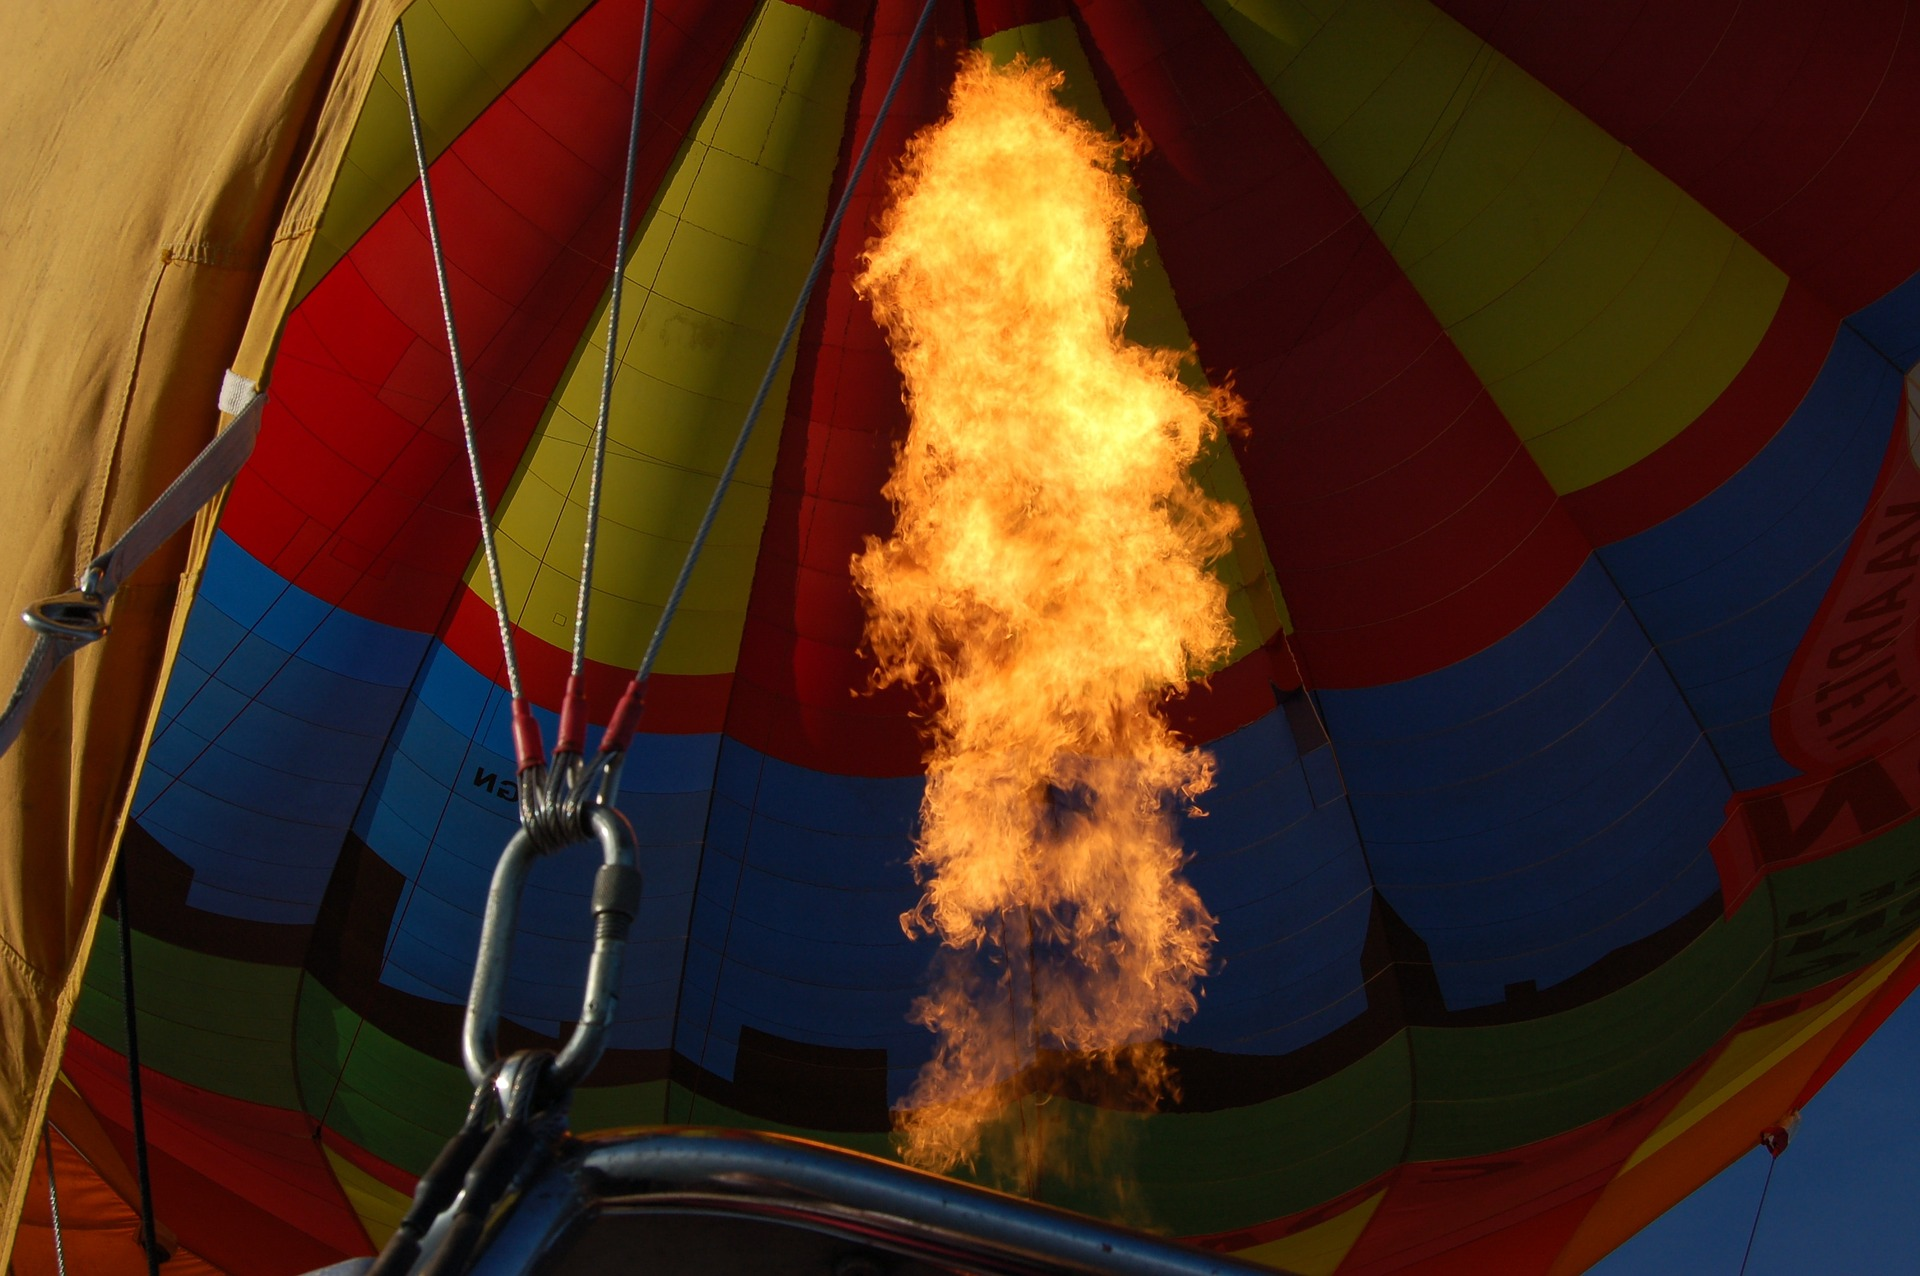
\includegraphics[width=\textwidth]{figures/balloon_burner.jpg}
    \caption{Example of a turbulent non-premixed flame: The burner of a hot air
    balloon.}
    \label{fig:balloon_burner}
\end{figure}
%

%
The effect of turbulence on the flame depends on the size and strength of
the eddies comprising the flow.
%
Large eddies move slowly and only wrinkle the surface in large scales.
%
This only has an indirect effect on the structure of the flame and the chemical
reactions, but influences the global flame shape.
%
Smaller eddies are faster and might disturb the structure of the flame locally.
%
This might have the effect of destroying a clean flame front and causing local
extinction, or it might enhance local mixing and improve the conditions for
combustion.
%
If the eddies are too small, they might be dissipated before they are able to
influence the reaction significantly.
%
Which scales interact with the flame in which way is also dependent on the speed
at which the chemical reaction happens, the flame thickness, and in the case of
premixed combustion, the flame speed.
%
Building accurate models for turbulent combustion requires in\-ves\-ti\-ga\-ting
the interplay of all these variables and more.
%
\subsubsection{Turbulent Premixed Flames} % (fold)
\label{ssub:turbulent_premixed_flames}
%
In premixed flames, turbulence has the primary effect of enhancing combustion.
%
The turbulent flow wrinkles the flame surface and increases its surface area.
%
A higher surface area means that reaction happens at more places at once.
%
The global flame speed increases and fresh gases are consumed more rapidly.
%
However, at high turbulence intensities, the heat produced by the reaction
will be dissipated too quickly and the flame might be extinguished.
%

%
Due to the massive change in viscosity on the burnt gas side, the turbulence
intensity in premixed flames is typically much stronger in the fresh gases.
%
This difference is so significant that the flow on the burnt gas side may become
laminarized, depending on the initial turbulence intensity.
%

%
In practice, premixed combustion occurs for example in spark-ignited internal
combustion engines.
%
Here, air-fuel mixture is sucked into the cylinder, compressed and then ignited.
%
Starting from the ignition point, the flame front travels through the cylinder,
being wrinkled by the turbulent flow of the gas and transforming all fresh gases
into hot combustion products.
%
% subsubsection turbulent_premixed_flames (end)
%
\subsubsection{Turbulent Diffusion Flames} % (fold)
\label{ssub:turbulent_diffusion_flames}
%
The typical diffusion flame setup is the jet flame.
%
A stream of fuel gas, often turbulent, is injected into ambient air.
%
Mixing between fuel and air is provided by the turbulent shear layer that arises
from the difference in velocities between the two gases.
%
This leads to a reaction zone that is typically very thin at the outlet and
becomes thicker as more mixing occurs downstream, where a substantial volume is
occupied by combustion products.
%
A practical example for a diffusion jet flame is shown in
\cref{fig:balloon_burner}.
%

%
A central problem of turbulent diffusion flames is flame stabilization.
%
Typically, combustion does not start directly after the fuel gas leaves the
inlet, but only after some mixing has occurred.
%
This mixed gas then needs to be ignited by already-burning mixture further
downstream.
%
This lateral propagation of the flame needs to happen at least at the same
velocity as the flow, otherwise the flame will be blown off.
%
To make this process more stable, some setups provide small premixed pilot
flames between fuel an air stream to provide a steady source of heat.
%

%
If mixing occurs faster than combustion, or if the flame is locally extinguished
due to high flame stretch, pockets of premixed gas can form that are later
ignited when coming into contact with high-temperature regions.
%
This means that parts of a diffusion flame might actually be in the premixed
regime.
%
This highlights the complexity of diffusion flames compared to premixed flames.
%
Due to the additional problem of mixing, diffusion flames are much more
sensitive to turbulence.
%
Depending on their setup, many different conditions and mechanisms can be in
effect at the same time.
%
This makes non-premixed flames very challenging to model and simulate.
%
% subsubsection turbulent_diffusion_flames (end)
%
% subsection turbulent_combustion (end)
%
% section combustion (end)
%
\section{Modeling and Simulation of Turbulent Combustion} % (fold)
\label{sec:simulation_of_turbulent_combustion}
%
% - Why simulation
% - simulation needs models
% - Turbulent combustion needs models from both turbulence and combustion
% - Both complex and computationally expensive
% - Combination even more expensive
% - Assumptions and simplifications necessary to make things more performant
% - Which assumptions can be made under what circumstances subject to ongoing
%   research
% - Provide overview of modelling strategies for chemistry and turbulence
% - Focus on DNS as it is most relevant for this thesis
Simulations are used to make predictions about the behavior of a system.
%
In turbulent combustion and other engineering application they provide a
quick and cheap way of testing setups compared to setting up experiments.
%
A simulation is only useful if it is sufficiently accurate.
%
This is why good models of the underlying processes are so important.
%
On the other hand, simulations also need to be efficient.
%
If running the simulation is more expensive and time-consuming than setting up
a comparable experiment, the simulation loses much of its value.
%

%
For turbulent combustion, finding a good trade-off between accuracy and
efficiency is very much an open problem.
%
Both turbulent flow and chemical reactions are complex to model and expensive
to simulate on their own.
%
Solving both at once in a turbulent combustion simulation predictably leads to
a vast increase in the required computing time and resources.
%
Frequently simplifying assumptions are made to gain efficiency.
%
Which assumptions are valid under which circumstances is the central question
when building turbulent combustion models.
%

%
This section provides an overview of modeling strategies used in turbulent
combustion simulations.
%
It places a particular focus on \acl{DNS}, as it is most relevant for the
content of this thesis.
%
\subsection{Chemical Schemes} % (fold)
\label{sub:chemical_schemes}
%
Modeling a chemical reaction can be a complex task.
%
Most reactions do not consist of a single step but rather a complex system of
intermediate reactions.
%
Many of these reactions can be reversible and their reaction rates depend on the
current composition and temperature of the gas.
%
The more complex the fuel, the more intermediate steps are possible and need to
be considered when modeling the reaction.
%
A system of intermediate steps that models a whole reaction is called a chemical
scheme (see, \eg, \cref{tab:hydrogen_scheme}).
%
Each individual reaction step has a number of parameters controlling the
reaction rate in dependence on the current temperature.
%
\begin{table}[t]
    \caption[Example scheme for \ce{H2}-\ce{O2} combustion]
            {Example scheme for a seemingly simple chemical reaction: Hydrogen
             and Oxygen react to produce water \cite{Miller1982}. \ce{M} is a
             placeholder for a third molecule that is needed to absorb and
             dissipate excess energy to stabilize the product.}
    \label{tab:hydrogen_scheme}
    \centering
    \begin{tabularx}{\linewidth}{lX}
    \toprule
    \textbf{Elements:} & \ce{H},  \ce{O},  \ce{N} \\
    \midrule
    \textbf{Species:} & \ce{H2}, \ce{O2}, \ce{OH}, \ce{O}, \ce{H}, \ce{H2O},
                        \ce{HO2}, \ce{H2O2}, \ce{N2}\\
    \midrule
    \textbf{Reactions:} &
    {$\begin{aligned}
        \ce{H2 + O2 &<=> 2 OH} & \ce{2 OH &<=> O + H2O}\\
        \ce{H2 + OH &<=> H2O + H} & \ce{H2 + M &<=> 2 H + M}\\
        \ce{H + O2 &<=> OH + O} & \ce{O2 + M &<=> 2 O + M}\\
        \ce{O + H2 &<=> OH + H} & \ce{H + OH + M &<=> H2O + M}\\
        \ce{H + O2 + M &<=> HO2 + M} & \ce{HO2 + H &<=> H2 + O2}\\
        \ce{H + 2 O2 &<=> HO2 + O2} & \ce{2 HO2 &<=> H2O2 + O2}\\
        \ce{H + O2 + N2 &<=> HO2 + N2} & \ce{H2O2 + M &<=> 2 OH + M}\\
        \ce{OH + HO2 &<=> H2O + O2} & \ce{H2O2 + H &<=> H2 + HO2}\\
        \ce{H + HO2 &<=> 2 OH} & \ce{H2O2 + OH &<=> H2O + HO2}\\
        \ce{O + HO2 &<=> O2 + OH} &
    \end{aligned}$}\\
    \bottomrule
    \end{tabularx}
\end{table}
%

%
Reaction modeling is the task of breaking down the wealth of possible
intermediate reactions into a subset that describes the whole reaction with
sufficient accuracy for a given application, and determining the right
parameters for each one.
%
For complex hydrocarbon fuels the number of different species considered
can easily go into the hundreds, while thousands of intermediate steps
contribute to the reaction.
%
Even for seemingly simple reactions, such as Hydrogen and Oxygen to Water,
the reaction schemes can be surprisingly complex.
%
The scheme by Miller \etal~\cite{Miller1982} displayed in
\cref{tab:hydrogen_scheme} has 9 species and 19 different reactions.
%
Adding this to an already computationally intensive fluid dynamics simulation
that only involves five different variables (density, temperature and three
velocity components) increases the computational load immensely.
%
This is amplified even more by the fact that chemical reactions, especially the
intermediate ones in a reaction scheme, typically happen at much smaller time
scales than the flow.
%
This means that compared to non-reacting flows, not only do the number of
equations and variables increase immensely, but the simulation time steps also
become much smaller.
%

%
There are some strategies to increase efficiency.
%
The simplest one is to use single-step chemistry.
%
Here, the reaction is assumed to be infinitely fast and the flame front to be
infinitely thin.
%
Fuel and oxidizer are immediately transformed into products and heat once the
conditions for combustion are met.
%
In this case, no intermediate reactions are considered, which greatly decreases
the number of variables and equations to solve and allows larger time steps.
%
Due to the strong assumptions made when using this method, the results can be
very inaccurate, but it can be useful to get a qualitative result.
%
More accurate but also more expensive methods precompute a lookup table covering
the relevant portion of the parameter space or reduce the parameter space to
lower-dimensional manifolds.
%
Explaining these methods in detail is out of the scope of this work.
%

%
Modeling chemical reactions is a complex field in its own right.
%
Turbulent combustion researchers mostly use existing chemical libraries and
schemes in their codes.
%
Often, the trade-off between accuracy and efficiency has to lean heavily towards
efficiency to keep simulation times and memory usage in a reasonable range.
%
% subsection chemical_schemes (end)
%
\subsection{The Flamelet Assumption} % (fold)
\label{sub:the_flamelet_assumption}
%
Moving from reactions to turbulent flames, we need a model for the structure
of the flame.
%
The most common assumption is that the flame front is thin compared to the
scales of the turbulent eddies.
%
This means that the flame front can be approximated by an iso-surface of the
reaction progress variable in the case of premixed flames or the mixture
fraction for diffusion flames.
%
Assuming a thin flame front allows to treat the turbulent flame like a set of
locally laminar flames, so-called \emph{flamelets}, that are wrinkled but not
disturbed by the flow.
%
Orthogonal to the surface, the flame is assumed to behave like the
\ac{1D} laminar equivalent.
%
Models for laminar combustion can then be directly used to determine the
behavior of the flame at each location on the idealized flame surface.
%
This includes models for the relationship between flame speed, flame stretch,
flame thickness, reaction rates, heat release and so on.
%

%
The flamelet assumption is frequent in combustion modeling, as it greatly
simplifies the flame structure and limits the effects of turbulence on the
behavior of the flame that need to be considered.
%
Of course, the conditions for this assumption are not always fulfilled:
%
\begin{itemize}
    \item
    %
    Parts of the flame might be locally quenched.
    %
    In the case of premixed flames, this allows fresh gases to penetrate into
    the burnt gas side and vice-versa, something that does not happen for
    laminar flames.
    %
    In the case of diffusion flames, this allows the formation of pockets of
    premixed gas that are later ignited and do not confirm to the ideal
    diffusion flame any more.
    %
    \item
    %
    The ideal flame front might be disturbed by small-scale mixing.
    %
    In this case, the flame structure can be very different than that of laminar
    flames.
    %
    The distinction between burnt/unburnt or fuel/oxidizer side becomes less
    clear and the flame structure can no longer be adequately described by a
    simple iso-surface.
\end{itemize}
%
Due to the simpler flame structure and the smaller sensitivity to turbulence,
the flamelet assumption is more often valid for premixed than for diffusion
flames.
%
More complex models that allow some interaction of turbulence with the
small-scale flame structure are subject of ongoing research.
%
% subsection the_flamelet_assumption (end)
%
\subsection{High-Level Models: \acs{RANS} and \acs{LES}} % (fold)
\label{sub:high_level_models}
%
\begin{figure}[t]
    \centering
    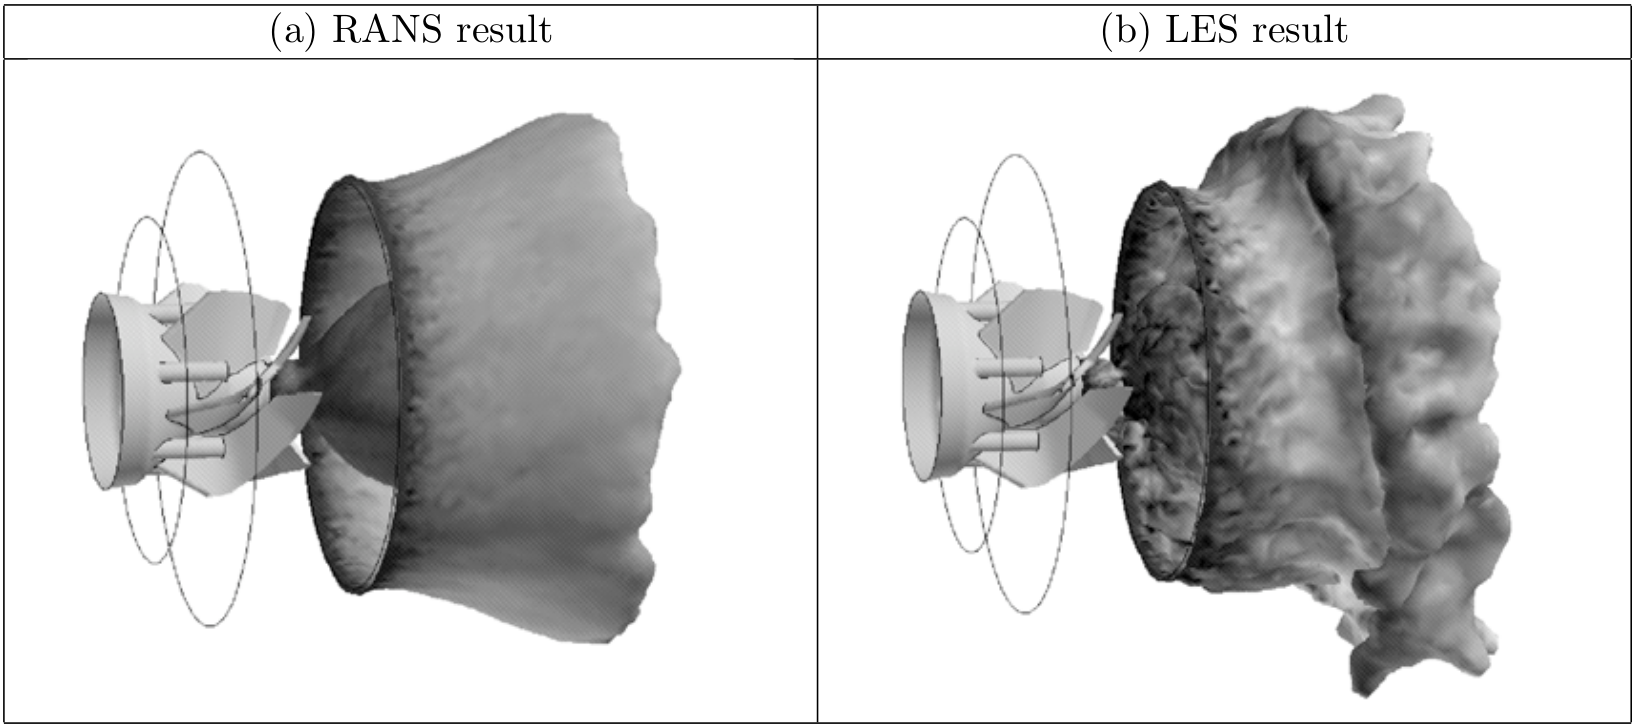
\includegraphics[width=\textwidth]{figures/rans_vs_les.png}
    \caption{Comparison of temperature iso-surfaces in a swirled combustor when
    using \ac{RANS} and \ac{LES}. Image source: Poinsot and Veynante
    \cite{Poinsot2012}}
    \label{fig:rans_vs_les}
\end{figure}
%
Computational fluid dynamics (\acs{CFD}\acused{CFD}) knows three main categories
of models for simulating turbulent flow.
%
They are, in decreasing order of abstraction, \acf{RANS}, \acf{LES} and
\acf{DNS}.
%
For simulating turbulent combustion, these are extended by combustion models
according to their character.
%
The first part of this thesis focuses heavily on \ac{DNS}, which is discussed in
detail in the next section.
%
Since \ac{DNS} is one of the main tools for validating and building \ac{RANS}
and \ac{LES} models, we will briefly discuss the ideas behind both here.
%
\subsubsection{Reynolds-Averaged Navier-Stokes} % (fold)
\label{ssub:rans}
%
\acl{RANS} simulates the time-averaged, steady-state behavior of the system.
%
It is based on the decomposition of the behavior of a turbulent system into
averaged and fluctuating parts.
%
The result are average values for all simulation variables at each location.
%
Images of \ac{RANS} simulations show very smooth fields that have almost no
small-scale features (see \eg, \cref{fig:rans_vs_les}).
%

%
Combustion models for \ac{RANS} can be based on quantities such as the mean
flame surface area per unit volume, turbulent mixing rates, or probability
density functions based on one-point statistics.
%

%
Since \ac{RANS} simulations do not resolve unsteady effects, their results have
to be interpreted with care.
%
Mean values reported by \ac{RANS} say nothing about the possibly large
fluctuations that occur there.
%
However, \ac{RANS} is the most popular and widespread method for simulating
turbulent combustion because of its low computational cost.
%
% subsubsection rans (end)
%
\subsubsection{Large Eddie Simulations} % (fold)
\label{ssub:les}
%
A step up from \ac{RANS} in terms of accuracy and computational cost are
\ac{LES}.
%
They reproduce unsteady, but low-pass filtered effects of the system.
%
The simulation runs on a lower-resolution grid and only resolves the larger
scales explicitly.
%
Small-scale sub-grid effects are modeled.
%
\ac{LES} produce an unsteady, but "blurry" representation of reality (see
\cref{fig:rans_vs_les}).
%

%
Combustion models for \ac{LES} face the challenge that the flame front is
generally much smaller than the grid resolution.
%
Combustion phenomena that control the evolution of the flame front happen almost
exclusively at sub-grid scales.
%
\ac{LES} approaches deal with this by describing the flame front in terms of
some filtered variable that can be resolved on the grid.
%
Some approaches artificially thicken the flame front, others assume the
flame front as an iso-surface of some smooth variable.
%
In any case, small-scale wrinkling of the flame front cannot be resolved in
\ac{LES} and needs to be expressed via models.
%

%
With the increase in computing performance in recent years, \ac{LES} has gained
popularity and is seeing more widespread use.
%
However, \ac{LES} of turbulent combustion is still maturing, and accurate
sub-grid models for combustion are the subject of ongoing research.
%
% subsubsection les (end)
%
% subsection high_level_models_for_turbulent_combustion_ac (end)
%
\subsection{Direct Numerical Simulations} % (fold)
\label{sub:direct_numerical_simulations}
%
The most accurate and detailed numerical results in \ac{CFD} are produced by
\ac{DNS}.
%
In these simulations, all time and length scales are resolved on a regular grid.
%
On this grid, the Navier-Stokes equations are solved directly without using a
model for turbulence.
%
This produces an accurate representation of reality, which is why \ac{DNS} is
also often referred to as a ``numerical experiment''.
%

%
Its brute-force approach means that \ac{DNS} is conceptually relatively simple
compared to \ac{RANS} and \ac{LES}, but it is the most demanding of the three
in terms of computational resources and time.
%
As a consequence, \ac{DNS} are typically used only for small domains of a few
centimeters at most.
%
Although methods for more complex setups and geometries are under active
development, the typical case is a rectangular box with simple boundary
conditions.
%
This is why non-reacting \ac{DNS} has typically been used to study turbulent
flows near walls, between parallel plates or behind simple rectangular
geometries.
%

%
Like for \ac{RANS} and \ac{LES}, the choice of chemistry model for \ac{DNS} is
largely dependent on the available computing resources and performance demands.
%
If we apply the ideal of solving everything without high-level models, then the
logical choice would be using complex chemistry with full chemical schemes.
%
Unfortunately, this is rarely feasible.
%
Even adding single-step chemistry to a non-reacting \ac{DNS} can result in a
hundred-fold increase in computing time due to the smaller time steps and grid
sizes required.
%
Using complex chemical schemes only amplifies this problem.
%
For complex fuels, the only choice for getting results in a reasonable time
frame is therefore to make a massive trade of accuracy in favor of performance.
%
Even then, turbulent combustion \ac{DNS} of non-trivial cases can only be run
on large supercomputers using thousands of parallel cores.
%

%
Despite the large computational cost and restriction to simple case setups,
\ac{DNS} is an important tool for combustion modeling.
%
It provides high-resolution \ac{3D} unsteady data for all variables, which is
still impossible to obtain via experiments.
%
This data allows an in-depth analysis of the behavior of turbulent flames that
can be leveraged to build, validate and improve higher-level models.
%
\begin{figure}[t]
    \centering
    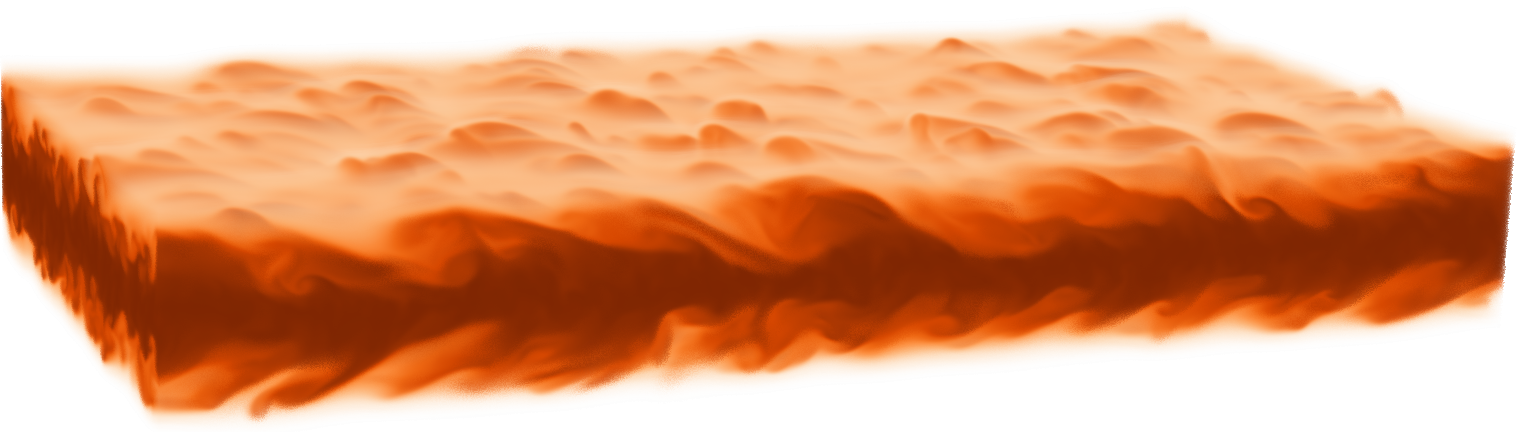
\includegraphics[width=\textwidth]{figures/Hawkes_VolRend.png}
    \caption{Direct volume rendering of the mixture fraction in a
    \ac{DNS} of a turbulent non-premixed flame.}
    \label{fig:turbulent_diffusion_flame_dns}
\end{figure}
%

%
\ac{DNS} is used mainly for two purposes:
%
Gaining data to validate and fine-tune \ac{RANS} and \ac{LES} models, and
gaining a deeper understanding of turbulence/chemistry interactions to derive
new models.
%
A wide variety of analysis approaches are applied to these effects.
%
These range from very simple validation by looking at aggregated quantities to
investigation of complex effects such as the different mechanisms for reignition
of locally extinguished parts of the flame.
%
Providing an exhaustive discussion would go beyond the scope of this chapter,
but we will take a look at some examples to get an idea of the kind of
properties that are investigated.
%

%
The simplest forms of analysis are applied for the validation of \ac{RANS} and
\ac{LES} models.
%
Here, the same case is simulated once using \ac{RANS} or \ac{LES}, and once
using \ac{DNS}.
%
Validation can happen at a high level by comparing aggregated quantities such as
the average or maximum temperatures, or on a lower level by comparing point-wise
quantities or statistics.
%
In this case it is important to take into account the differences in
representation between \ac{DNS} and the higher-level models.
%
In the case of \ac{RANS}, \ac{DNS} results have to be temporally averaged in
order to be meaningfully comparable.
%
For \ac{LES}, the \ac{DNS} data needs to be low-pass filtered before comparison.
%

%
More complex analysis is needed when checking the validity of basic assumptions
underlying the high-level models, such as the flamelet assumption.
%
In the case of \ac{RANS}, this can be done by computing different kinds of
statistics, depending on the combustion model used.
%
Simple point statistics can be computed without regard for the flame structure.
%
If the flame front is thin, flamelets may be extracted as profiles orthogonal
to an iso-surface representing the flame surface, or along trajectories of the
temperature or mixture fraction gradient.
%
Statistics may also be derived from ensembles of iso-levels of characteristic
variables such as temperature or mixture fraction.
%
The result are distributions as a function of this variable.
%
Finally, space-averaged statistics might be used to determine quantities such as
the average amount of flame surface area per unit volume.
%

%
Other quantities that are often investigated due to their significance in
combustion modeling are the flame speed (if applicable), thickness, surface
stretch and curvature.
%
The relationship of all of these quantities with the structure of the flame is
still not completely understood.
%
This is why \ac{DNS} results are frequently compared to laminar flames as a
baseline.
%
For example, Sankaran \etal \cite{Sankaran2007} analyzed the flame thickness and
curvature in a premixed jet flame statistically and compared the results to a
laminar flame.
%
Hawkes and Chen~\cite{Hawkes2006} investigated the statistical similarity of
methane-air flames in the ``thin reaction zones'' regime, which uses slightly
weaker assumptions than the flamelet regime, to strained laminar flames.
%
The approach presented in \cref{cha:sparse_representation} facilitates such
studies by providing a representation of a premixed flame from which such
statistics can readily be computed, as well as enhancing it by an additional
possibility of visual analysis.
%

%
A promising area of current research is concerned with the mechanisms of local
extinction and reignition and the effect of unsteady, non-instantaneous effects
on the flame.
%
These are especially interesting for diffusion flames, as they are more
sensitive to turbulence and local extinction has a major significance for the
applicability of flamelet models.
%
Many works in this area use Lagrangian approaches to study the temporal behavior
of flame elements.
%

%
Yeung \etal \cite{Yeung1990} tracked ensembles of points attached to material-
and flame surfaces in premixed and diffusion flames.
%
They recorded the histories of strain rates acting on these surface points to
determine under what circumstances a flame surface remains close to an initially
coincident material surface.
%
Statistics extracted from the ensemble of surface points allowed them to
determine in what way the flame surface grows or shrinks over time and how the
strain experienced by a flame surface element affects the flame dynamics.
%

%
Sripakagorn \etal \cite{Sripakagorn2004} tracked points attached to an
iso-surface of the mixture fraction over time to detect and classify local
extinction and reignition events.
%
They showed that extinction happens primarily if the flame surface is subject to
large amounts of strain over a certain time period.
%
They also identified three different mechanisms for reignition of previously
extinguished parts of the flame.
%

%
Scholtissek \etal \cite{Scholtissek2017} tracked complete flamelets represented
as trajectories of the mixture fraction gradient emanating from such points on
the mixture fraction iso-surface.
%
They analyzed the histories of these flamelets and derived a new flamelet model
that accounts for curvature-induced tangential transport between adjacent
flamelets.
%

%
Such Lagrangian approaches are becoming more prevalent in the combustion
community.
%
They provide an important tool for the derivation of new combustion models
that incorporate unsteady effects.
%
\Cref{cha:flame_surface_tracking} of this thesis presents an approach for
tracking the complete flame surface that is intended to support such
investigations in large-scale \ac{DNS}.
%
% subsection direct_numerical_simulations_for_turbulent_combustion (end)
%
% section modeling_and_simulation_of_turbulent_combustion (end)
%
\section{Visualization for \ac{DNS} of Turbulent Combustion} % (fold)
\label{sec:visualization_for_dns_of_turbulent_combustion}
%

%
\subsection{Post Processing} % (fold)
\label{sub:post_processing}
%

%
% subsection post_processing (end)
%
\subsection{In-Situ Approaches} % (fold)
\label{sub:in_situ_approaches}
%

%
% subsection in_situ_approaches (end)
%
% section visualization_for_dns_of_turbulent_combustion (end)
%
% chapter turbulent_combustion (end)
